\section{Interfaccia Utente}
L'obiettivo dell'interfaccia utente era fornire una visualizzazione chiara e intuitiva dei meeting programmati. 
A tal fine, è stato scelto un calendario come elemento principale dell'interfaccia.
\\\\
In particolare, si è deciso di utilizzare \textit{FullCalendar} \cite{FullCalendarSite},
una famosa libreria Javascript open source che si integra perfettamente con React.
\\\\
Grazie al \textbf{MUI Theme}, l'utente ha la possibilità di personalizzare i colori 
principali del sito a proprio piacimento tramite una pratica interfaccia laterale:
\begin{figure}[H]
    \centering
    % Figura impostazioni tema - chiaro
    \begin{minipage}{0.45\textwidth}
        \centering
        \includegraphics[width=\textwidth]{ThemeSettings/LightTheme.png}
        \caption{Tema chiaro}
    \end{minipage}
    \hspace{0.05\textwidth}
    % Figura impostazioni tema - scuro
    \begin{minipage}{0.45\textwidth}
        \centering
        \includegraphics[width=\textwidth]{ThemeSettings/DarkTheme.png}
        \caption{Tema scuro}
    \end{minipage}
\end{figure}
\clearpage
\noindent Un esempio di visualizzazione della pagina utilizzando entrambi i temi:
% Visualizzazione calendario mensile tema chiaro
\begin{figure}[H]   
    \centering
    \includegraphics[width=\textwidth]{VisualizzazioneCalendario/LightTheme.png}
    \caption{Visualizzazione Calendario - tema chiaro}
    \label{fig:visualizzazioneCalendario}
\end{figure}
% Visualizzazione calendario mensile tema scuro
\begin{figure}[H]
    \centering
    \includegraphics[width=\textwidth]{VisualizzazioneCalendario/DarkTheme.png}
    \caption{Visualizzazione Calendario - tema scuro}
\end{figure}
\noindent Per far capire che un evento è concluso, viene mostrato con uno sfondo grigio.
\noindent  Nel caso siano presenti più eventi in un giorno nella visualizzazione mensile 
del calendario, è possibile utilizzare un pratico popup per avere una visione migliore:
\begin{figure}[H]
    \centering
    % Figura impostazioni tema - chiaro
    \begin{minipage}{0.45\textwidth}
        \centering
        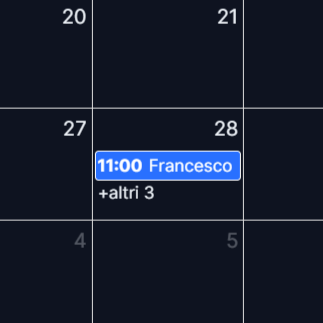
\includegraphics[width=0.5\textwidth]{VisualizzazioneCalendario/+Meet.png}
        \caption{+ altri meet}
    \end{minipage}
    \hspace{0.05\textwidth}
    % Figura impostazioni tema - scuro
    \begin{minipage}{0.45\textwidth}
        \centering
        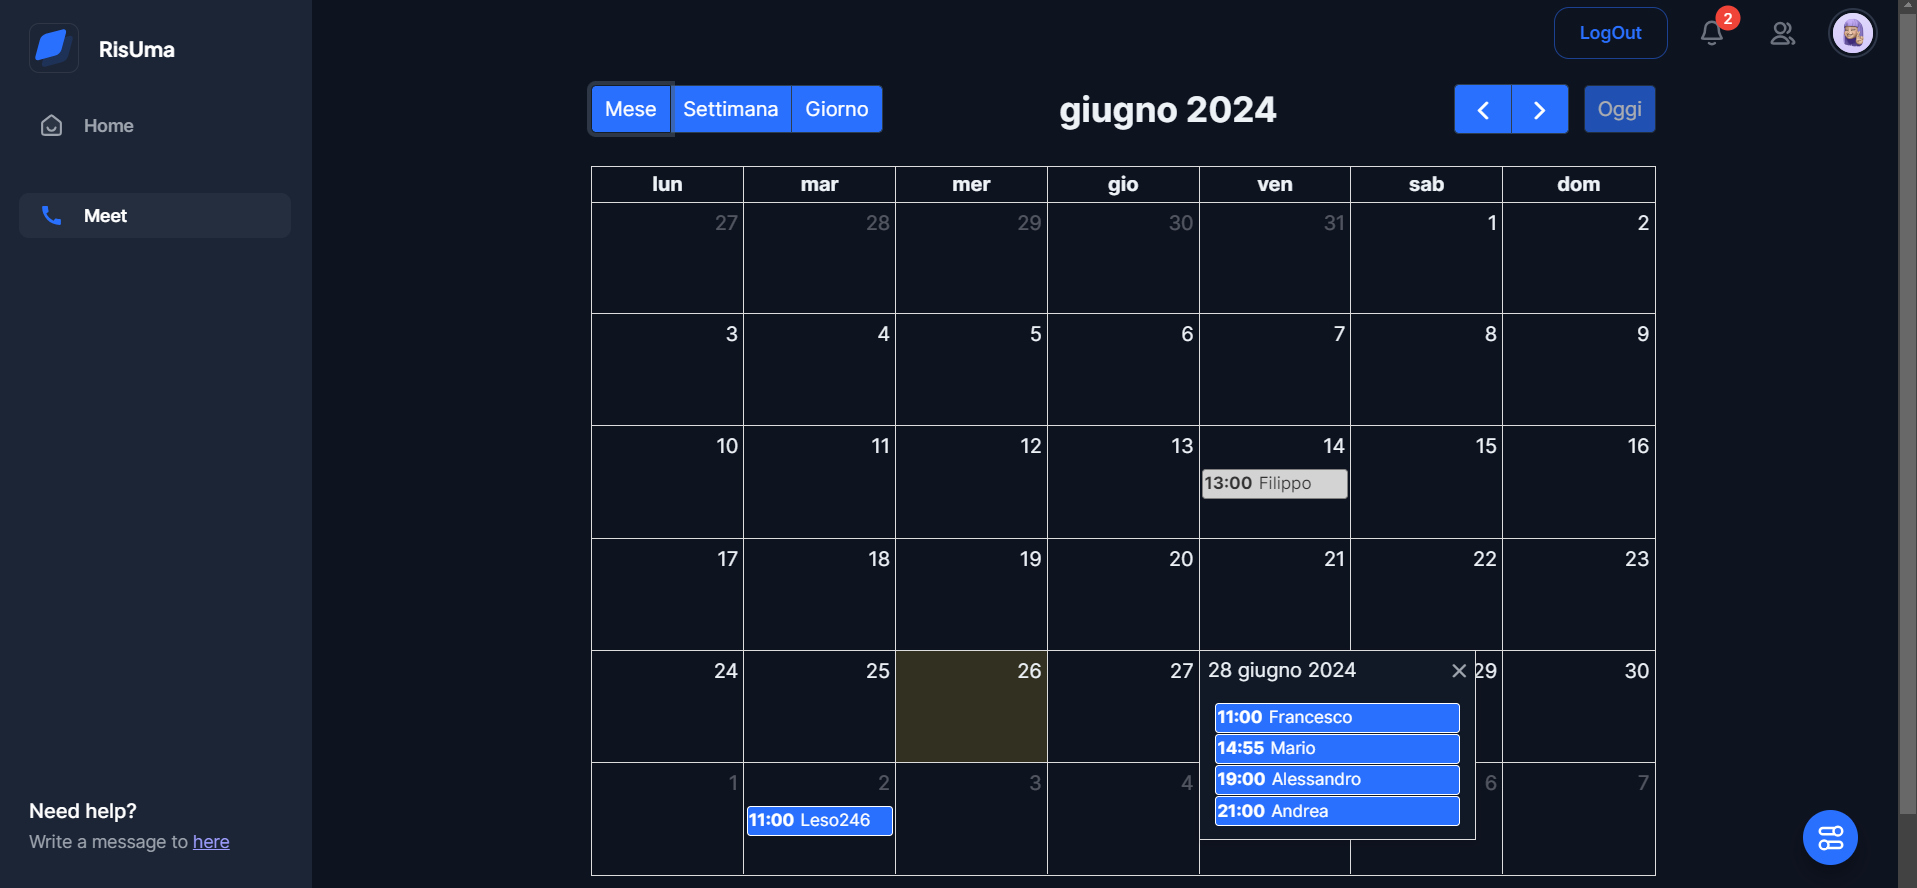
\includegraphics[width=\textwidth]{VisualizzazioneCalendario/popup+MeetDark.png}
        \caption{popup meet}
    \end{minipage}
\end{figure}
\clearpage
\noindent È anche disponibile una visualizzazione settimanale e giornaliera:
\begin{figure}[H]
    \centering
    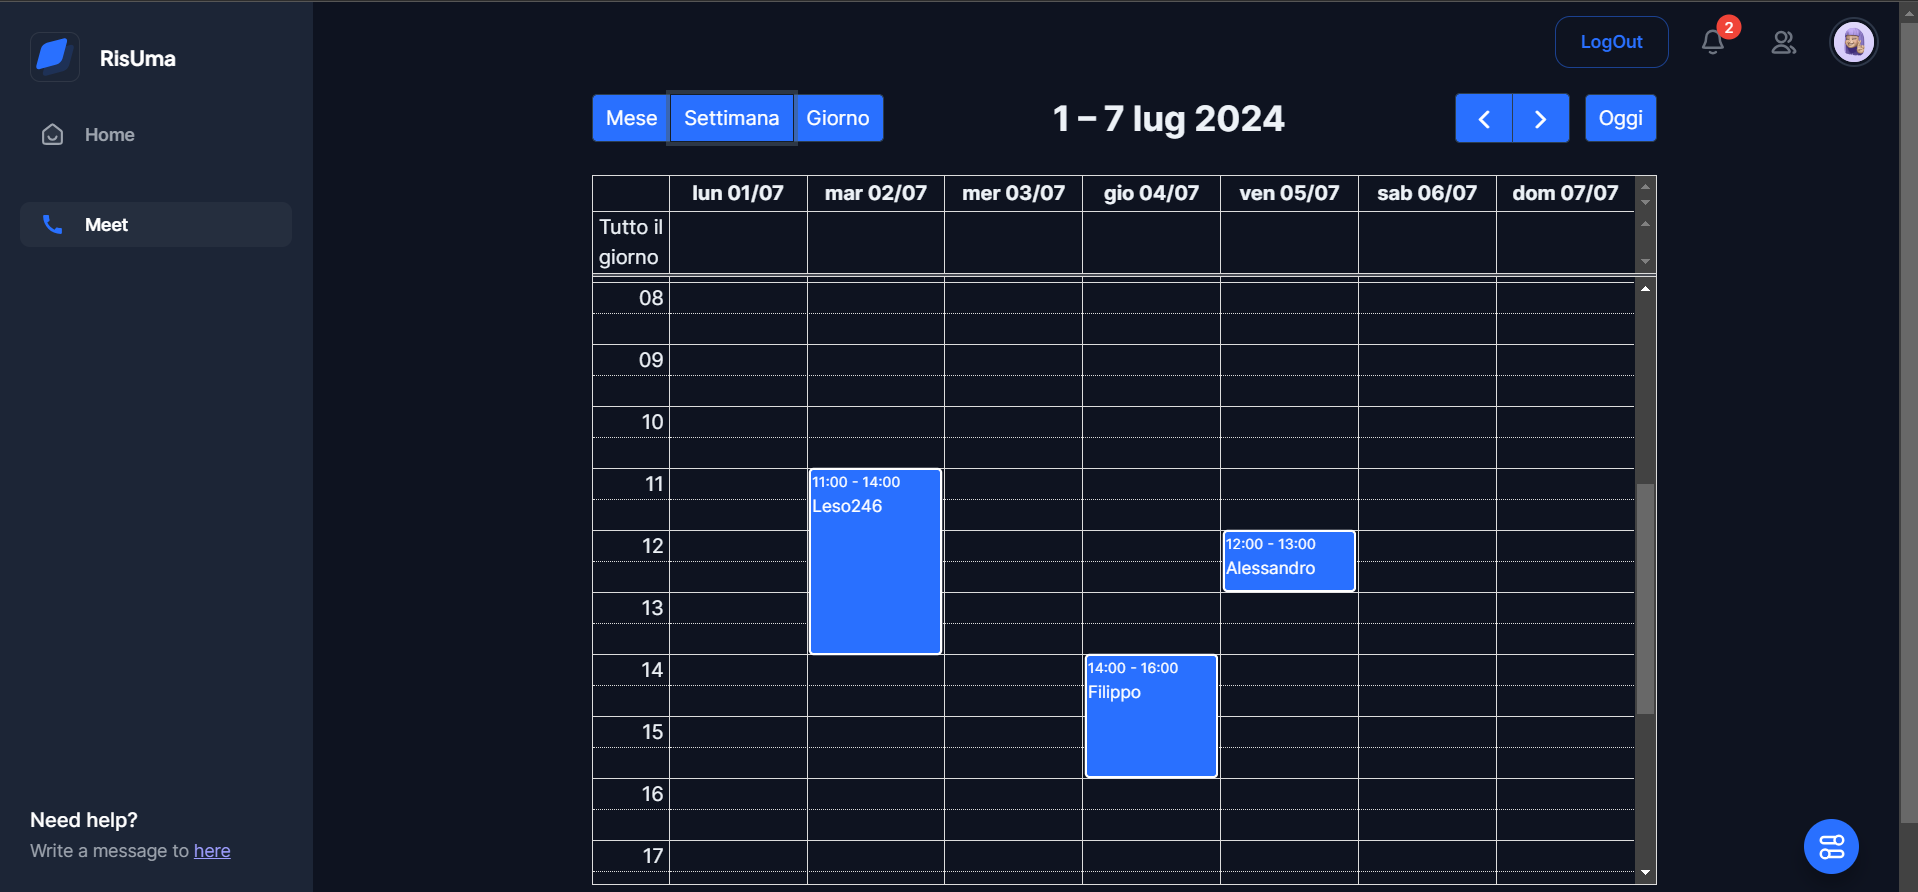
\includegraphics[width=\textwidth]{VisualizzazioneCalendario/VisualizzazioneSettimana.png}
    \caption{Visualizzazione Settimanale - tema scuro}
\end{figure}
\begin{figure}[H]
    \centering
    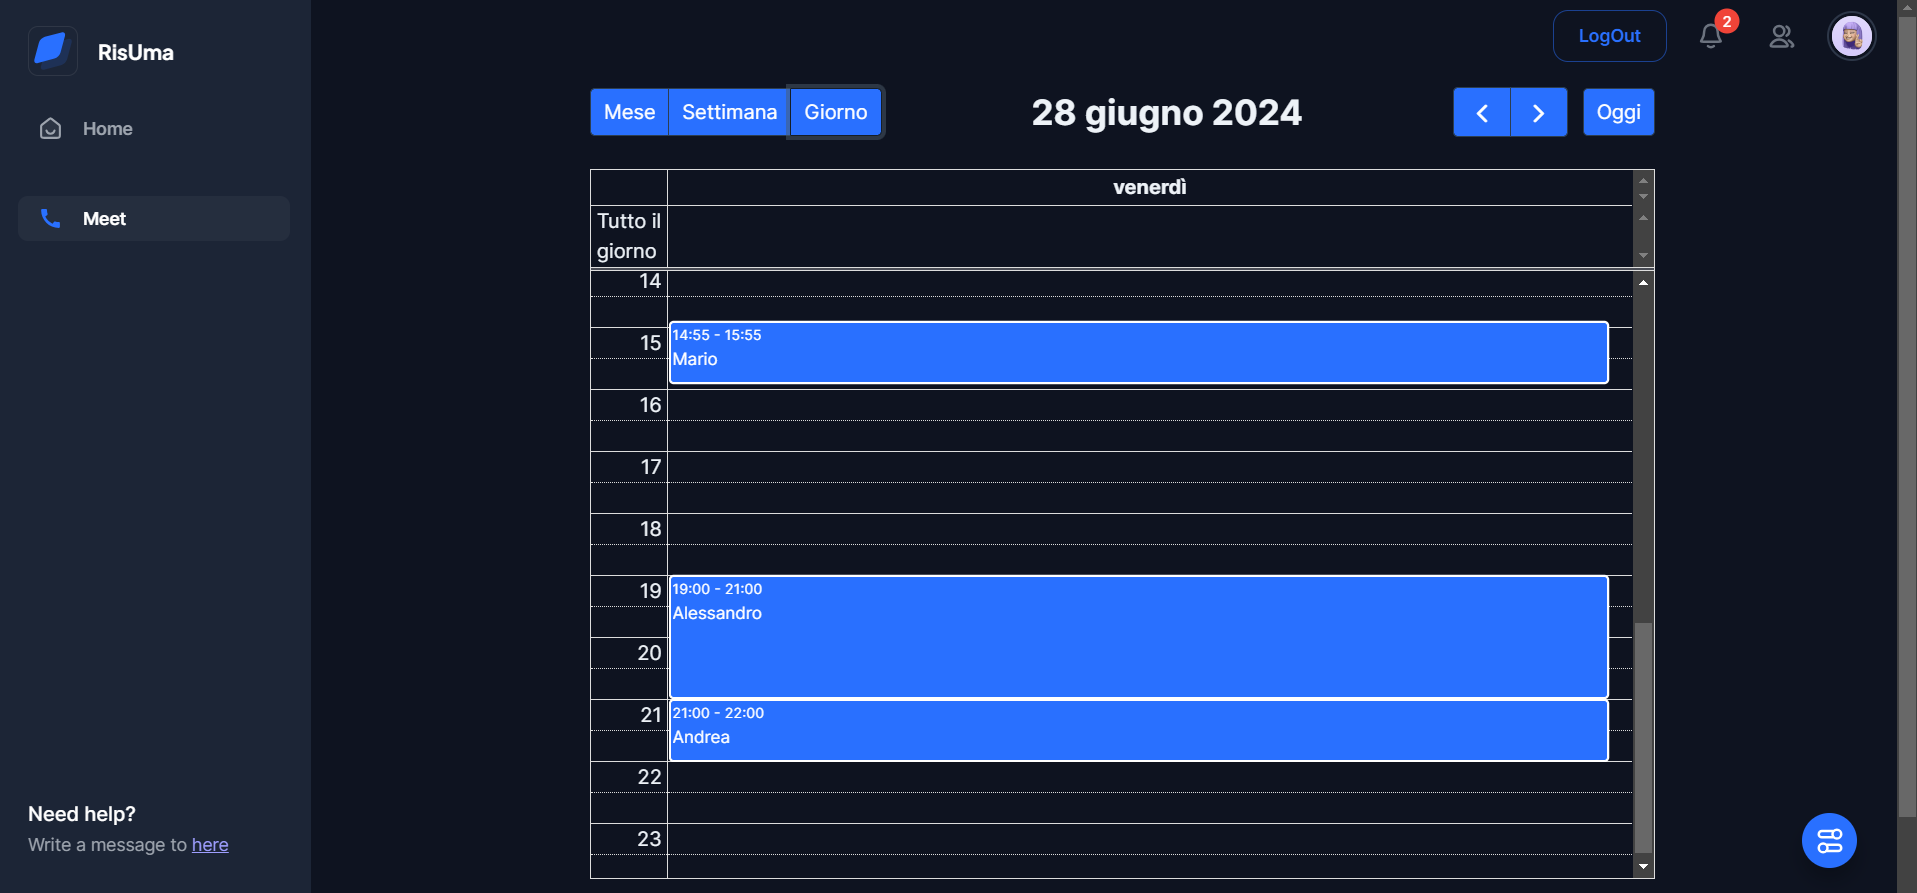
\includegraphics[width=\textwidth]{VisualizzazioneCalendario/VisualizzazioneGiorno.png}
    \caption{Visualizzazione Giornaliera - tema scuro}
\end{figure}
\noindent In seguito si entrerà nel dettaglio dei restanti elementi dell'interfaccia utente.